\section{HARP extension for flexible performance-complexity balancing}\label{sec:our-method}

While the prolongation used by HARP is sufficient when used only as a means of pre-training, the approach is far too crude when studying the relationship between graph complexity and the quality of graph embedding as a single coarsening iteration can reduce the number of nodes to less than half. In order to overcome this limitation, we present the adaptive prolongation approach. This algorithm works with the pre-coarsened graphs produced by HARP, however, the embedding is learned in a different manner. The \( L \) coarsening steps are decoupled from \( K \) prolongation steps, where \( K \) is independent of \( L \). The prolongation steps are then driven by local properties of the graph with relation to the downstream task, allowing for different levels of granularity in different parts of the graph.

\begin{figure}
	\centering
	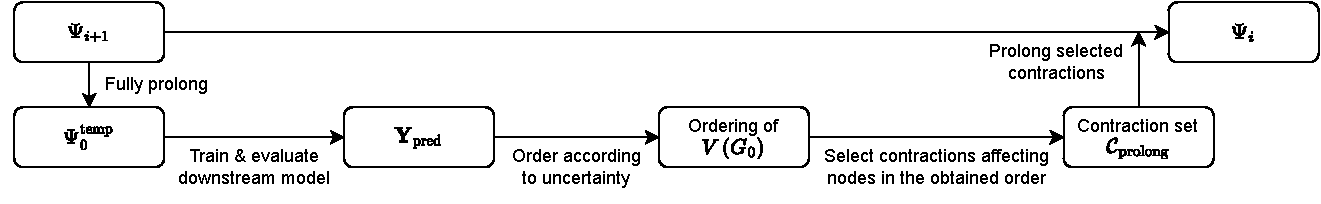
\includegraphics[width=\textwidth]{images/adaptive-prolongation/adaptive-prolongation.pdf}
	\caption{A schematic explanation of the adaptive prolongation algorithm for obtaining the embedding \( \Psi_{i} \) from \( \Psi_{i + 1} \).}
	\label{fig:adaptive-prolongation}
\end{figure}

Let us denote \( \Psi_K, \dots, \Psi_0 \) the resulting embedding sequence. Similarly to standard HARP prolongation, the algorithm starts with the coarsest graph \( G_L \), trains a graph model to compute its embedding \( \Psi_K \) and gradually refines it until reaching the embedding \( \Psi_0 \). These prolongation steps are interlaid with continued training of the graph model, as in standard HARP. A description of a single prolongation step from \( \Psi_{i + 1} \) to \( \Psi_i \) follows and is schematically outlined in Figure~\ref{fig:adaptive-prolongation}.

The procedure keeps track of all the edge contractions that were made in the dataset augmentation part of the algorithm and gradually reverses them. To this end, apart from the embedding \( \Psi_i \), the set of all contractions yet to be reversed as of step \( i \) is kept as \( \mathcal{C}_L^{(i)}, \dots, \mathcal{C}_0^{(i)} \), with the initial values \( \mathcal{C}_j^{(K)} \) corresponding to the underlying coarsening \( \varphi_j \) as defined in Section~\ref{sec:harp}.

In each prolongation step, the embedding \( \Psi_{i + 1} \) is prolonged to \( \Psi_i \) by selecting a set of \( n_p \) contractions \( \mathcal{C}_\mathrm{prolong} \) and undoing them by copying and reusing the embedding of the node resulting from the contraction to both of the contracted nodes. To obtain \( \mathcal{C}_\mathrm{prolong} \), nodes of \( G_0 \) are first ordered in such a way that corresponds to the usefulness of prolonging them. Subsequently, the set \( \mathcal{C}_\mathrm{prolong} \) is selected from \( \mathcal{C}_L^{(i + 1)}, \dots, \mathcal{C}_0^{(i + 1)} \) by selecting contractions affecting nodes in the aforementioned order, until \( n_p \) contractions are selected. If multiple contractions affecting the same node are available in the sequence \( \mathcal{C}_L^{(i + 1)}, \dots, \mathcal{C}_0^{(i + 1)} \), one is selected from \( \mathcal{C}_j^{(i + 1)} \) corresponding to the coarsest-level coarsening. The sequence \( \mathcal{C}_L^{(i)}, \dots, \mathcal{C}_0^{(i)} \) is produced from \( \mathcal{C}_L^{(i + 1)}, \dots, \mathcal{C}_0^{(i + 1)} \) by removing all of the edges contained in \( \mathcal{C}_\mathrm{prolong} \).

To obtain an ordering of nodes of \( G_0 \) based on the usefulness of their prolongation, the embedding \( \Psi_{i + 1} \) is fully prolonged to a temporary embedding of the full graph, \( \Psi_0^\mathrm{temp} \). The downstream model is then trained using this temporary embedding to obtain \( \mathmat{Y}_\mathrm{pred} \), the predicted posterior distribution of classes for each node in \( G_0 \). The nodes are ordered by the entropy of the posterior, making the algorithm prolong the nodes where the classifier is the most uncertain.
